% main.tex
% Fichero principal de transparencias (incluye a todos los demás).

% Compilar a .pdf con LaTeX (pdflatex)
% Es necesario instalar Beamer (paquete latex-beamer en Debian)
%

% Gráficos:
% Los gráficos pueden suministrarse en PNG, JPG, TIF, PDF, MPS
% Los EPS deben convertirse a PDF (usar epstopdf)
%
\documentclass[17pt,aspectratio=169,hyperref=pdfusetitle]{beamer}
\usetheme[orchid]{Hannover}
\beamertemplatenavigationsymbolsempty
\setbeamertemplate{headline}{}
\useoutertheme{infolines}

\usepackage[spanish]{babel}
\usepackage[utf8]{inputenc}
\usepackage{graphics}
%\usepackage{amssymb} % Simbolos matematicos
%\usepackage[pdfusetitle]{hyperref}

\usepackage{chronosys}

%% two slides per page
%\usepackage{pgfpages}
%\pgfpagesuselayout{2 on 1}[a4paper,border shrink=5mm]

\newcommand\YUGE{\fontsize{48}{60}\selectfont}

\newcommand{\secimage}{figs/bookpages}
\AtBeginSection[]
{
  {
    \usebackgroundtemplate{\includegraphics[width=\paperwidth,height=\paperheight]{\secimage}}
    \begin{frame}<beamer>

      \begin{center}
        {\YUGE\bf\insertsection}
      \end{center}
    \end{frame}
  }
  \renewcommand{\secimage}{figs/bookpages}
}


\title[¿Controlas la tecnología...?]{La tecnología... \\ ¿la controlamos o nos controla?}
%\subtitle{}
\author[Jesús M. González Barahona]{\small Jesús M. González Barahona //
@jgbarah}
\institute[URJC]{Universidad Rey Juan Carlos}
  %\url{http://github.com/jgbarah/presentations}


\date[III Jornada TIC y sostenibilidad]{\small III Jornada sobre TIC y Sostenibilidad \\ El lado oscuro de la tecnología \\
  Internet, 3 de noviembre de 2020}

\begin{document}

%\begin{frame}[label=firstframe]
\begin{frame}
  \maketitle
\end{frame}

%%---------------------------------------------------------------

\begin{frame}
\frametitle{La tecnología permite y limita...}

\begin{flushright}
La tecnología nos permite hacer cosas nuevas \\
o nos limita \\
dependiendo de su arquitectura básica \\
(técnica, legal, económica) \\
\vspace{.2cm}
Su impacto (social, personal) \\
puede ser enorme y muy diferente \\
\end{flushright}

\end{frame}

%%---------------------------------------------------------------

\begin{frame}
\frametitle{...pero no suele ser parte del debate social}

\begin{center}
{\Large
Raramente reflexionamos\\
personalmente, socialmente, \\
políticamente, \\
sobre ello \\
}
\end{center}

\end{frame}

%%---------------------------------------------------------------

\begin{frame}

\begin{center}
{\Huge
Hoy toca... \\
(por un rato) \\
}
\end{center}

\end{frame}


%%-----------------------------------------
\begin{frame}[fragile]
  \frametitle{Internet nos salió rana}

  ~
  \vspace{2cm}
  \begin{flushright}
  \includegraphics[width=6cm]{figs/salir-rana}
  \end{flushright}

\end{frame}


%%-----------------------------------------
\begin{frame}[fragile]

  \begin{center}
  \includegraphics[width=7.5cm]{figs/apology-internet}
  \end{center}

  \begin{flushright}
    {\small
      \href{http://nymag.com/selectall/2018/04/an-apology-for-the-internet-from-the-people-who-built-it.html}{An Apology for the Internet from the People who Built It}
    }
  \end{flushright}

\end{frame}


%%-----------------------------------------
\begin{frame}[fragile]
  \frametitle{Internet es una gran oportunidad}


\end{frame}


%%-----------------------------------------
\begin{frame}[fragile]

  \begin{center}
  
\includegraphics[width=7.5cm]{figs/WSIS-Declaration-Principles}
  \end{center}

  \begin{flushright}
    {\small
      \href{http://www.itu.int/net/wsis/docs/geneva/official/dop.html}{Building the Information Society: a global challenge in the new Millennium}
    }
  \end{flushright}

\end{frame}


%%-----------------------------------------
\begin{frame}[fragile]
  \frametitle{¿Cómo puede ser una cosa y la contraria?}


\end{frame}

%%-----------------------------------------
\begin{frame}[fragile]
  \frametitle{La tecnología no es neutra}

  \begin{center}
  \includegraphics[width=10cm]{figs/code-is-law}
  \end{center}

\end{frame}

%%-----------------------------------------
\begin{frame}[fragile]
  \frametitle{Algunos ejemplos}


\end{frame}
%%---------------------------------------------------------------

\begin{frame}
\frametitle{Servicios de comunicación}

  \begin{itemize}
  \item Centralizado: un servicio \\
    para dominarlos a todos... \\
    (Facebook, Twitter, Hangouts, Whatsapp)
  \item Federado: múltiples proveedores de servicio, \\
    pero todos interoperan \\
    (correo electrónico, teléfono)
  \item Extremo a extremo: sin proveedores \\
    (IPFS, otros protocolos p2p)
  \end{itemize}

  \begin{flushright}
¿Cuál se puede controlar mejor? \\

¿En cuál se puede innovar mejor? \\

    ¿Cuál se puede adaptar mejor? \\
    \end{flushright}

\end{frame}

%%---------------------------------------------------------------

\begin{frame}
\frametitle{Servicios de comunicación}

\begin{flushright}
  {\Large
    ¿Cuál se puede controlar mejor? \\

    \vspace{.5cm}
    
    ¿En cuál se puede innovar mejor? \\

    \vspace{.5cm}

    ¿Cuál se puede adaptar mejor? \\
  }
    \end{flushright}

\end{frame}

%%-----------------------------------------
\begin{frame}[fragile]

  \begin{center}
  \includegraphics[width=10cm]{figs/home-assistants}
  \end{center}

  \begin{flushright}
    {\em
      \href{https://www.wired.com/2016/12/alexa-and-google-record-your-voice/}{Alexa and Google Home Record What You Say.} \\
      Wired \\
      }
  \end{flushright}
  
\end{frame}


%%---------------------------------------------------------------

\begin{frame}
\frametitle{Asistentes personales}

\begin{flushright}
  Google Now, Siri, Cortana (y muchos otros)
\end{flushright}

\begin{quote}
  ``Te aviso:
  ve saliendo para el aeropuerto \\
  porque tu avión despega en tres horas \\
  y hay un buen atasco en la M-40'' \\
\end{quote}


 {\small \href{http://searchengineland.com/how-google-now-siri-cortana-predict-what-you-want-229799}{How Google Now, Siri and Cortana predict...}}
\end{frame}


%%---------------------------------------------------------------

\begin{frame}
\frametitle{Mi coche tiene software}

Sólo quien puede cambiarlo puede...

\begin{itemize}
\item ...repararlo
\item ...adaptarlo a mis necesidades
\item ...decidir cómo se comporta
\end{itemize}

¿Quién decide si...

\begin{itemize}
\item ...puedo ser trazado en mis viajes?
\item ...mi coche puede matarme?
\end{itemize}

\end{frame}

%%-----------------------------------------
\begin{frame}[fragile]

  \begin{center}
  \includegraphics[width=12cm]{figs/tesla}
  \end{center}

  \begin{flushright}
    {\em
      \href{https://www.theverge.com/2017/9/10/16283330/tesla-hurricane-irma-update-florida-extend-range-model-s-x-60-60d}{The Verge} \\
      }
  \end{flushright}
  
\end{frame}


%%---------------------------------------------------------------

\begin{frame}
\frametitle{¿Quién decide qué puedes leer, qué puedes ver?}

\begin{center}
\includegraphics[height=4cm]{figs/tetasxtetas}
\end{center}

  \begin{flushright}
    {\small \url{https://youtu.be/vOP9hEhYCek}}
  \end{flushright}
\end{frame}


%%---------------------------------------------------------------

\begin{frame}
\frametitle{¿Cuál es el problema?}

{\large
\begin{center}
No es que una empresa \\
haga estas cosas
\pause
\vspace{1cm}

Es que se puedan hacer
\pause
\vspace{1cm}

y que socialmente dejemos que se hagan
\end{center}
}
\end{frame}

%%-----------------------------------------
\begin{frame}[fragile]
  \frametitle{Los tiempos están cambiando...}

\begin{columns}
  \begin{column}{0.7\textwidth}
    {\Large ¿Cuál será \\
    el próximo modelo \\
    de Internet? \\ }
  \end{column}
  \begin{column}{0.3\textwidth}  %%<--- here
    \begin{center}
      \includegraphics[width=\textwidth]{figs/The_Times_They_Are_a_Changin}
    \end{center}
  \end{column}
\end{columns}
  
\end{frame}


%%-----------------------------------------
\begin{frame}[fragile]
  \frametitle{Conocer es poder}

  \begin{center}
  
\includegraphics[width=9cm]{figs/switching-software}
  \end{center}

  \begin{flushright}
      \url{https://switching.software/} \\
  \end{flushright}

\end{frame}



%% ---------------------------------------------------------------

\begin{frame}
\frametitle{Una visión alternativa}

\begin{itemize}
\item Más cómputo, más almacenamiento, \\
  menos consumo, más movilidad \\
\item Más interconexión, más rápida, \\
  más barata \\
\item Mejores tecnologías federadas, \\
  extremo a extremo \\
\end{itemize}

  \begin{flushright}
  ¿Dispositivos personales
  interconectados directamente? \\
  \end{flushright}

\end{frame}

%% -----------------------------------------
\begin{frame}[fragile]
  \frametitle{Raspberry Pi 4}

  \begin{center}
  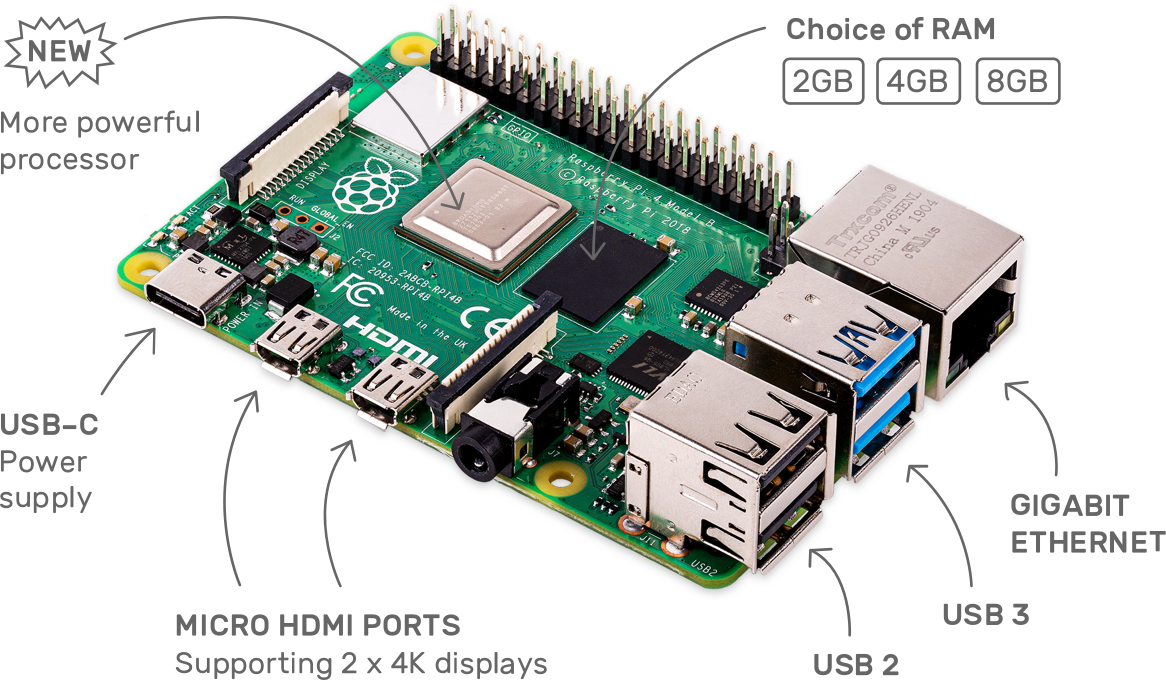
\includegraphics[width=10cm]{figs/raspberry-pi}
  \end{center}


\end{frame}


%%-----------------------------------------
\begin{frame}[fragile]

  \begin{center}
  \includegraphics[width=10cm]{figs/nextcloud}
  \end{center}
  
\end{frame}


%% -----------------------------------------
\begin{frame}[fragile]

  \begin{center}
  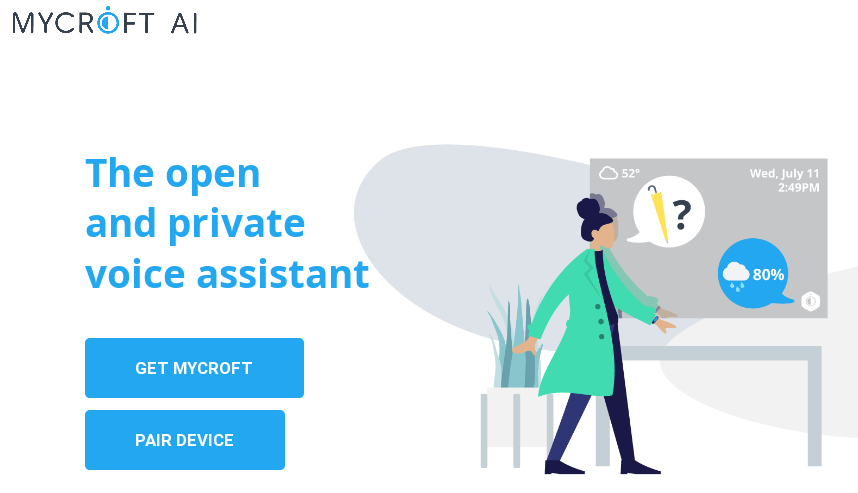
\includegraphics[width=10cm]{figs/mycroft}
  \end{center}

  \begin{flushright}
    {\em
      \href{https://mycroft.ai}{Mycroft}
      }
  \end{flushright}
  
\end{frame}


%%-----------------------------------------
\begin{frame}[fragile]
  \frametitle{Nada está garantizado}

  ``The coming war on general computation'', \\
  Cory Doctorow \\

  \url{https://youtu.be/HUEvRyemKSg}
\end{frame}

%%-----------------------------------------
\begin{frame}[fragile]

  {\em
  ``Freedom in the future will require us to have the capac­i­ty to mon­i­tor our devices and set mean­ing­ful pol­i­cy on them, to exam­ine and ter­mi­nate the process­es that run on them, to main­tain them as hon­est ser­vants to our will, and not as trai­tors and spies work­ing for crim­i­nals, thugs, and con­trol freaks.''
  }

  \begin{flushright}
  {\small
    \url{http://opentranscripts.org/transcript/coming-war-general-computation/}
  }
  \end{flushright}
  
\end{frame}

%%-----------------------------------------
\begin{frame}[fragile]
  \frametitle{Para terminar}

  ¿Cuál será el próximo modelo de Internet?

  \vspace{2cm}
  
  [Rellene su respuesta aquí]
  
\end{frame}

\frame{
~
\vspace{1cm}

\begin{flushright}


\includegraphics[width=2.2cm]{figs/by-sa}
 \\

\begin{footnotesize}
\copyright 2018-2020 Jesús M. González Barahona. \\

\vspace{.4cm}

Algunos derechos reservados. Este artículo se distribuye bajo
la licencia ``Reconocimiento-CompartirIgual 4.0 Internacional'' de Creative Commons,
disponible en \\
{\scriptsize \url{http://creativecommons.org/licenses/by-sa/4.0/deed.es}} \\

\vspace{.4cm}

Este documento (o uno muy similar) está disponible en \\
\url{http://jgbarah.github.io/presentations}

\end{footnotesize}
\end{flushright}

}
%%

%\againframe{firstframe}

\end{document}
